% !TEX root = main.tex

\section{Experiments}

\subsection{Fit Knowledge Base}

\begin{figure*}[!]
    \centering
    % \vspace{-0.2em}
    \begin{subfigure}[]{0.33\textwidth}
        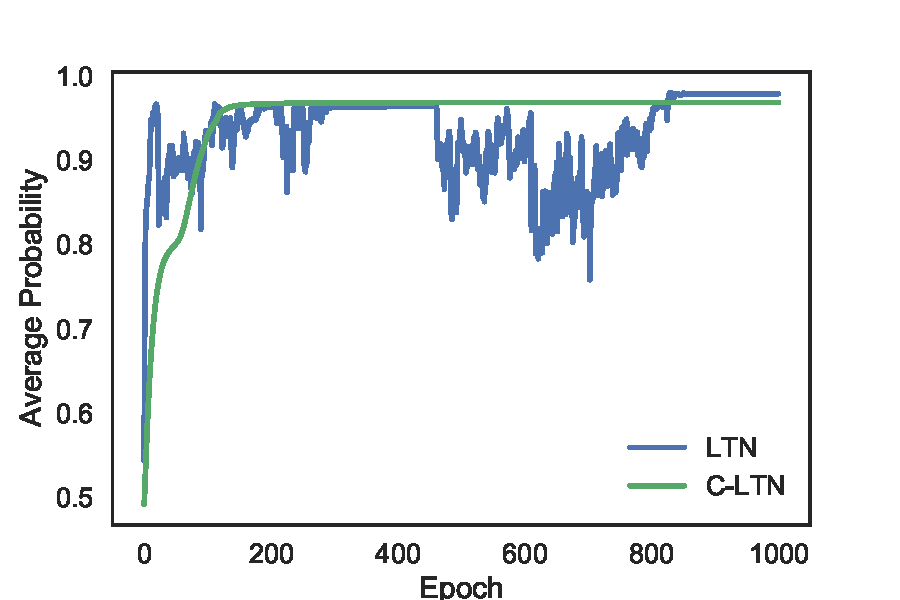
\includegraphics[width=\textwidth]{img/curve1.pdf}
        \caption{Probability w.r.t. Epoch}
        \label{fig:fitting-prob-epoch}
        %\vspace{-0.3em}
    \end{subfigure}~~~~
    \begin{subfigure}[]{0.33\textwidth}
        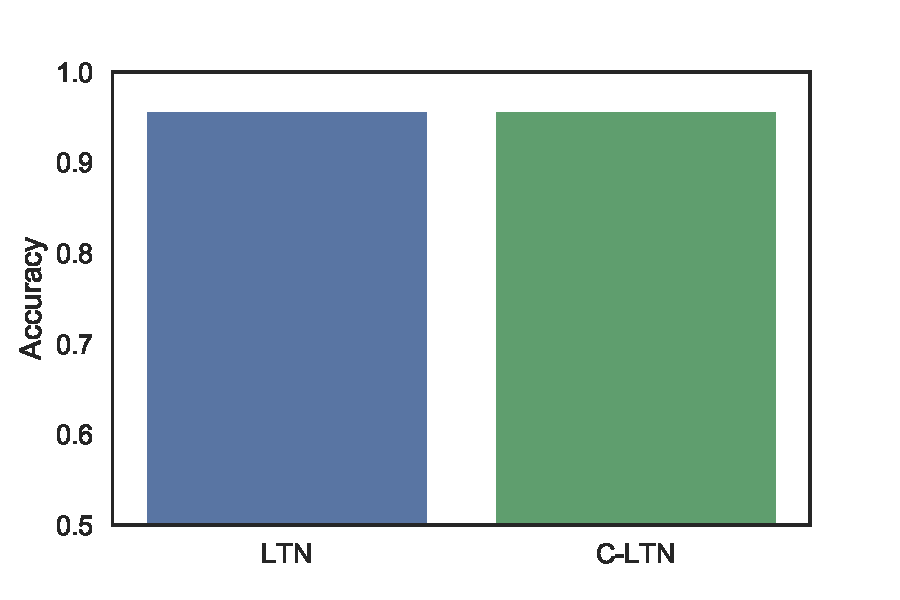
\includegraphics[width=\textwidth]{img/bar1.pdf}
        \caption{Best Accuracy on Group1}
        \label{fig:fitting-best-accuracy-1}
        %\vspace{-0.3em}
    \end{subfigure}~~~~
    \begin{subfigure}[]{0.33\textwidth}
        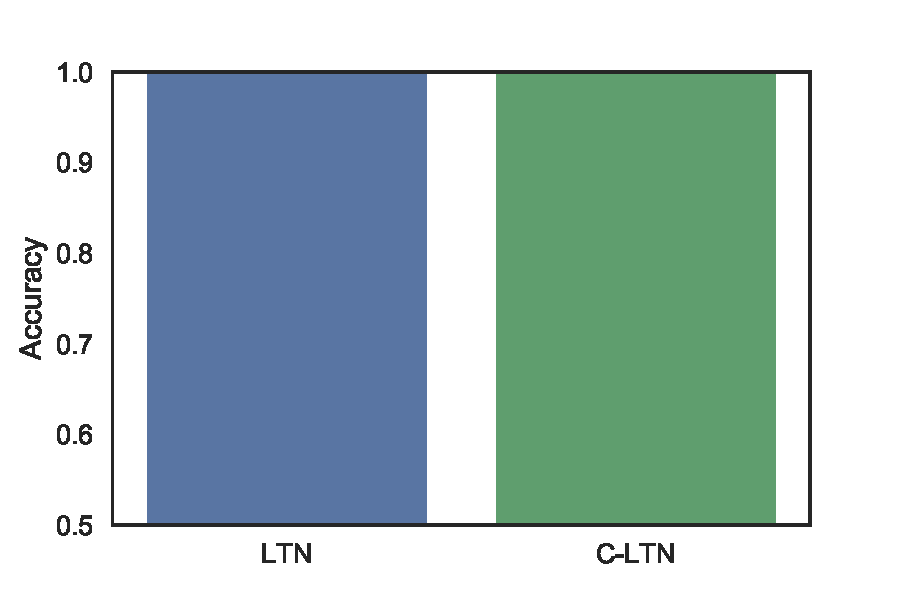
\includegraphics[width=\textwidth]{img/bar2.pdf}
        \caption{Best Accuracy on Group2}
        \label{fig:fitting-best-accuracy-2}
        %\vspace{-0.8em}
    \end{subfigure}
    \caption{Fitting Observed Facts.}
    \label{fig:fitting}
    % \vspace{-1.2em}
\end{figure*}

\subsection{Learn From Rule}

\begin{figure*}[!]
    \centering
    % \vspace{-0.2em}
    \begin{subfigure}[]{0.33\textwidth}
        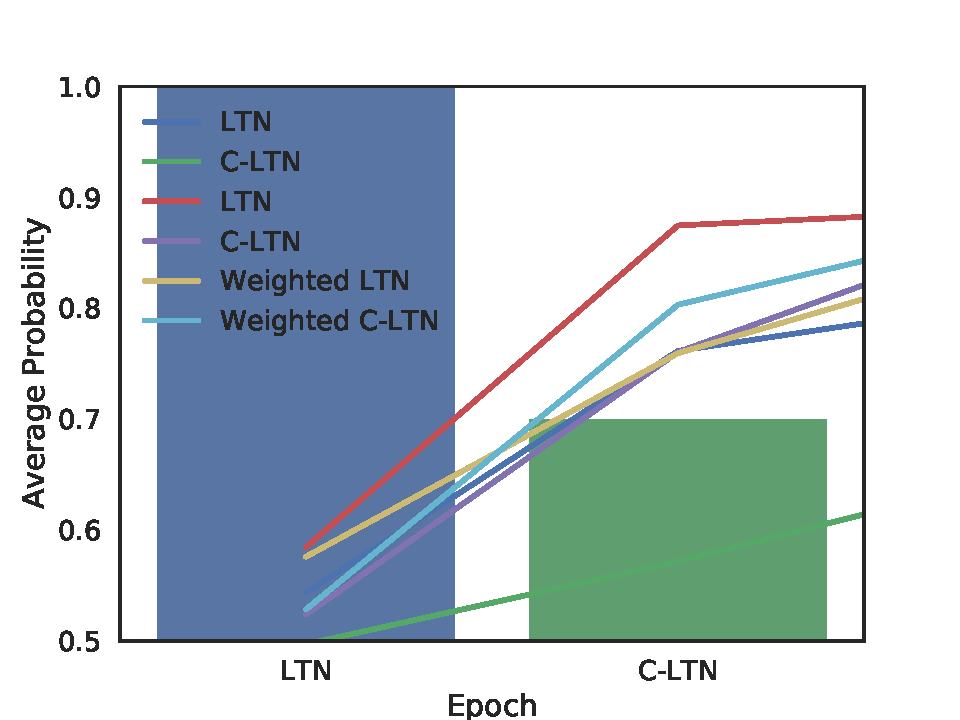
\includegraphics[width=\textwidth]{img/curve2.pdf}
        \caption{Probability w.r.t. Epoch}
        \label{fig:learning-prob-epoch}
        %\vspace{-0.3em}
    \end{subfigure}~~~~
    \begin{subfigure}[]{0.33\textwidth}
        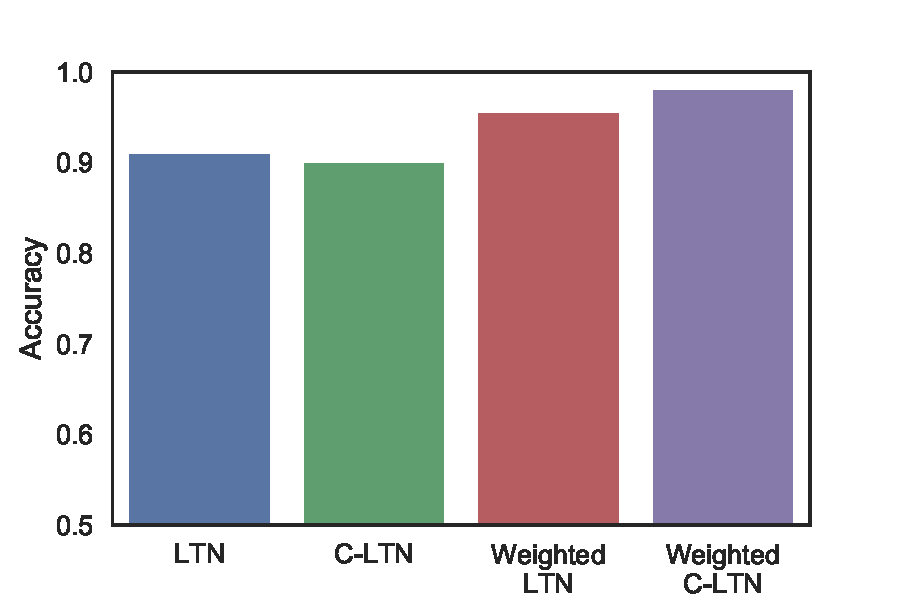
\includegraphics[width=\textwidth]{img/bar3.pdf}
        \caption{Best Accuracy on Group1}
        \label{fig:learning-best-accuracy-1}
        %\vspace{-0.3em}
    \end{subfigure}~~~~
    \begin{subfigure}[]{0.33\textwidth}
        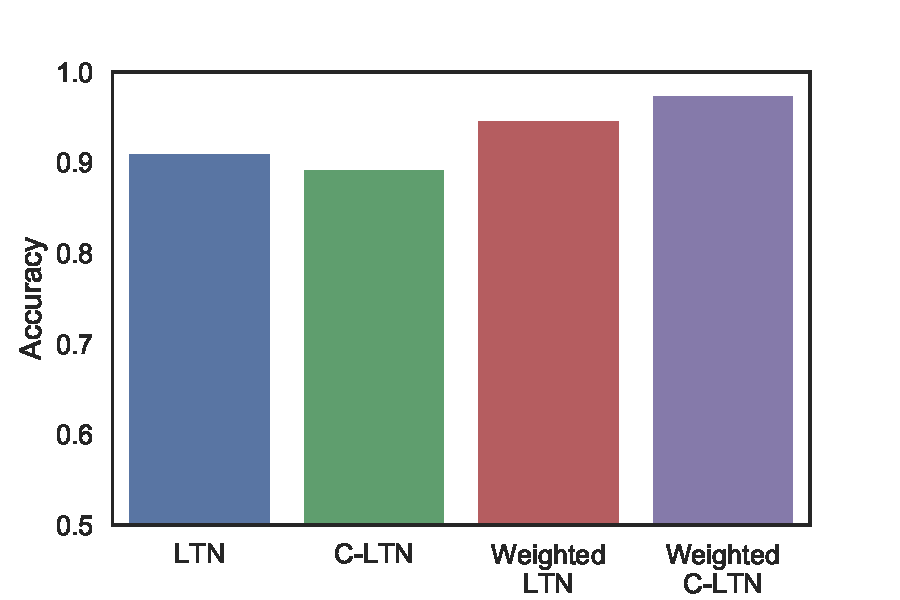
\includegraphics[width=\textwidth]{img/bar4.pdf}
        \caption{Best Accuracy on Group2}
        \label{fig:learning-best-accuracy-2}
        %\vspace{-0.8em}
    \end{subfigure}
    \caption{Learning from Observed Facts \& Rules.}
    \label{fig:learning}
    % \vspace{-1.2em}
\end{figure*}

\subsection{Parameter Sensitive}

\begin{figure}[!]
    \centering
    % \vspace{-0.2em}
    \begin{subfigure}[]{0.5\textwidth}
        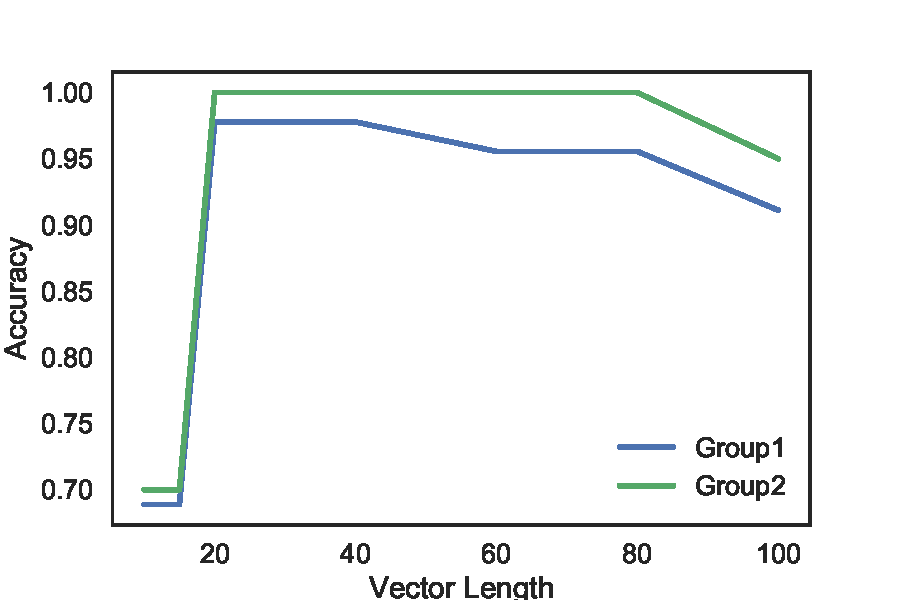
\includegraphics[width=\textwidth]{img/curve3.pdf}
        \caption{Fitting Observed Facts}
        \label{fig:sensitive-best-accuracy-1}
        %\vspace{-0.3em}
    \end{subfigure}

    \begin{subfigure}[]{0.5\textwidth}
        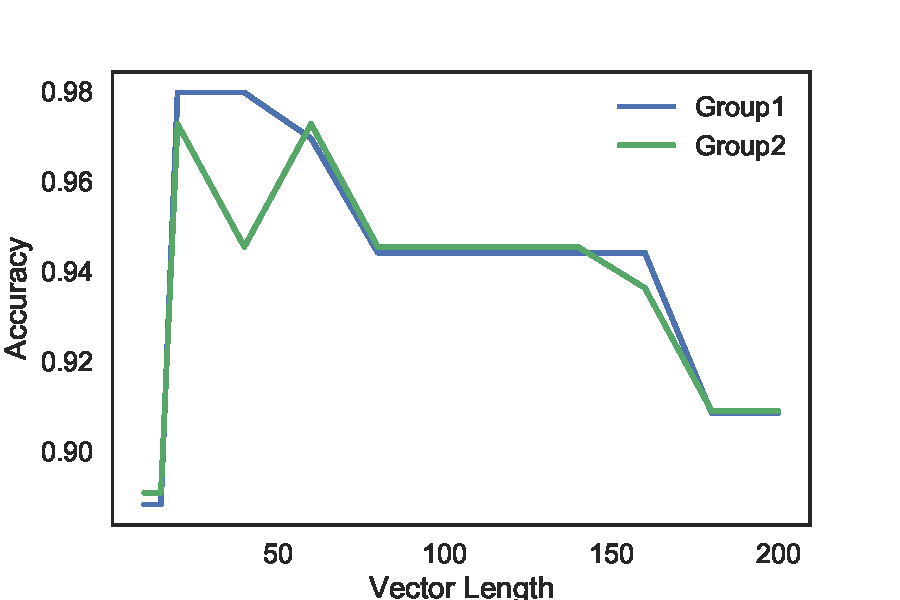
\includegraphics[width=\textwidth]{img/curve4.pdf}
        \caption{Learning from Rules }
        \label{fig:sensitive-best-accuracy-2}
        %\vspace{-0.3em}
    \end{subfigure}
    \caption{Best Accuracy w.r.t. Vector Length.}
    \label{fig:sensitive}
    % \vspace{-1.2em}
\end{figure}
